\subsection{Crystal Structures} \label{chap1}

First of all we need to identify in which structure calcium crystallizes.
As it can be seen in \autoref{tab:StructuresAndCellDimension_Table1_2_Omar},
it crystallizes in a FCC-structure.

\begin{table}[H]
	\centering
	\caption{Structures and Cell Dimensions of some Elements and Compounds,\\
	Elementary Solid State Physics \cite{elementary_SSP}, p. 18}
	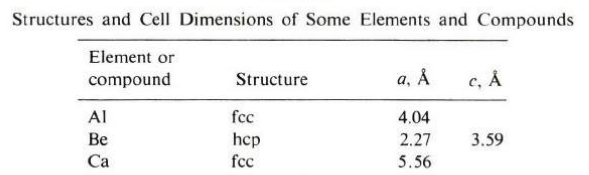
\includegraphics[width=0.5\linewidth]{Graphics/Chapter1/StructuresAndCellDimension_Table1_2_Omar}
	\label{tab:StructuresAndCellDimension_Table1_2_Omar}
\end{table}

FCC stands for \textit{Face-centered cubic}, which means 
the Calcium crystal is built up uf cubes with atoms at each
corner and an atom in the middle of each of the six cube planes
(as shown in \autoref{fig:face-centered_cubic_lattice}).

\subsubsection*{Unit Cell}
The convential Unit Cell of a FCC lattice looks as follows:

\begin{figure}[H]
	\centering
	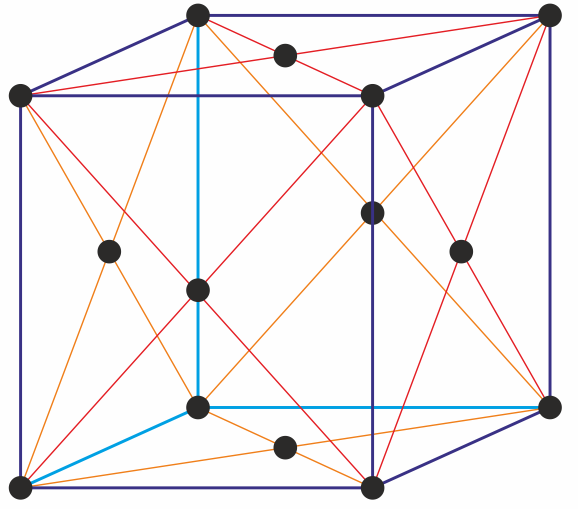
\includegraphics[width=0.4\linewidth]{Graphics/Chapter1/face-centered_cubic_lattice.png}
	\caption{FCC-Lattice}
	\label{fig:face-centered_cubic_lattice}
\end{figure}

\subsubsection*{Primitive Vectors}
With the primitive vectors each point in a lattice can be represented
by a linear combination of the three primitive vectors:

$$\mathbf{R} = n_1 \vec{u} + n_2 \vec{v} + n_3 \vec{w}$$

It may be said, that the lattice is invariant under the group of all 
translations expressed by $\mathbf{R}$.

The three primitive vectors for the FCC lattice are shown in 
\autoref{fig:prim_vec} and specified below.

\begin{figure}[H]
	\centering
	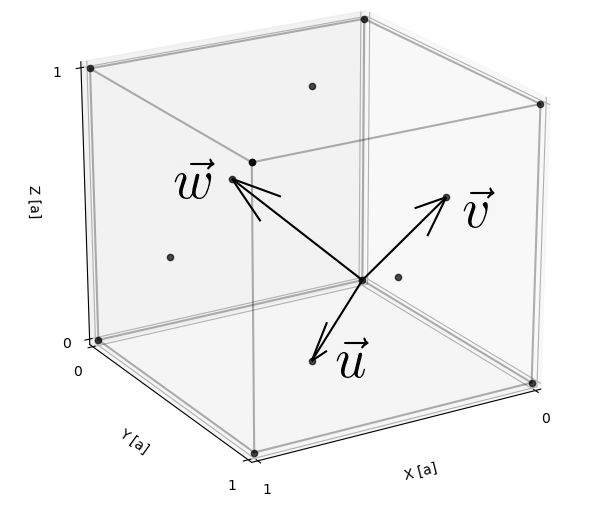
\includegraphics[width=0.5\linewidth]{Graphics/Chapter1/prim_vec}
	\caption{Primitive Vectors in a FCC-Lattice}
	\label{fig:prim_vec}
\end{figure}

\begin{equation}
	\vec{u} = \frac{a}{2} \left(\begin{matrix}1\\1\\0\\\end{matrix}\right) \qquad
	\vec{v} = \frac{a}{2} \left(\begin{matrix}0\\1\\1\\\end{matrix}\right) \qquad
	\vec{w} = \frac{a}{2} \left(\begin{matrix}1\\0\\1\\\end{matrix}\right)
	\label{eq:prim_vec}
\end{equation}


Whith these 3 base vectors a parallelepiped is given which is a primitive cell.
The volume of the primitive cell can be calculated with the following formula

$$V_{PC} = \vert (\vec{u} \times \vec{v})  \cdot \vec{w} \vert$$

which equals (with $a = 5.56 \, \mathring{A}$)

$$V_{PC} = \frac{a^3}{4} = 4.297 \cdot 10^{-30} \,m^3 = 4.297 \cdot 10^{-24} \,cm^3$$
\subsubsection*{Packaging Factor}

The Packaging Factor can be calculated as the ratio between the
volume of the atoms in the unit cell to the volume of the unit cell.

The volume of the unit cell can be calculated as:

$$V_{UC} = a^3$$


The unit cell containts 4 whole atoms.
One eighth of a atomic sphere at each corner (8) and one half at 
each cube face (6).

\begin{figure}[H]
	\centering
	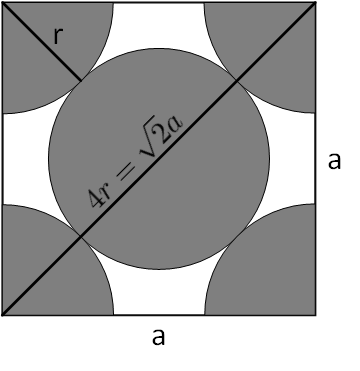
\includegraphics[width=0.3\linewidth]{Graphics/Chapter1/r_a_relation}
	\caption{Relation between the atomic radius and the parameter a in a FFC}
	\label{fig:r_a_relation}
\end{figure}

 As \autoref{fig:r_a_relation} shows the relationship between the parameter $a$ and the radius of the atomic sphere is given as:
$$r = \frac{\sqrt{2}}{4} a $$

And further the volume of the sphere

$$V_{Atom} = \frac{4}{3} \pi r^3 = \frac{a^3 \pi}{\sqrt{2^5}\cdot 3}$$

So the Atomic Packaging Factor $APF$ can be calculated as ratio between the
volume consumed by the atoms to the whole volume.

$$APF = \frac{4 \cdot V_{Atom} }{V_{UC}} = \frac{\pi}{3 \cdot \sqrt{2}} \approx 74\%$$


\subsubsection*{Density}

The atomic mass of calcium is given as \cite{lenntech_chemical_elements}:
$$m_{Ca} = 40.078 \frac{g}{mol}$$

By dividing the mass of the four atoms inside the FCC unit cell by the volume of the
unit cell we get the density of Calcium.

$$\rho = \frac{4}{N_A} \cdot \frac{m_{Ca}}{V_{UC}} = 1.55 \frac{g}{cm^3}$$

\subsubsection*{(110) Plane}

To show that the plane contains reticular rows of atoms in the specified
directions, we need to calculate the normal
vektor $\vec{n}$ of the plane, which we get by inverting the Miller Indices

$$\vec{n} = (\frac{1}{h} ,\, \frac{1}{k} ,\, \frac{1}{l}) = (1, \, 1,\, 0)$$

By knowing that the dot product between to orthogonal vectors is zero, we can show
that the three directions lay orthogonal to $\vec{n}$ and further so parallel
to the $(110)$ plane.

\begin{itemize}
	\item 	$[001]$\\
			$\vec{v_1} = (0, \, 0,\, 1)$\\
			$\vec{n} \cdot \vec{v_1} = 1 \cdot 0 + 1 \cdot 0 + 0 \cdot 1 = 0$
\end{itemize}
\begin{itemize}
	\item 	$[1\overline{1}0]$\\
			$\vec{v_1} = (1, \, -1,\, 0)$\\
			$\vec{n} \cdot \vec{v_1} = 1 \cdot 1 + 1 \cdot (-1) + 0 \cdot 0 = 0$
\end{itemize}
\begin{itemize}
	\item 	$[\overline{1}11]$\\
			$\vec{v_1} = (-1, \, 1,\, 1)$\\
			$\vec{n} \cdot \vec{v_1} = 1 \cdot (-1) + 1 \cdot 1 + 0 \cdot 1 = 0$
\end{itemize}

By knowing that the three directions lay inside or parallel to the plane, we
showed that the plane contains reticular rows of atoms in the $[001]$, $[1\overline{1}0]$
and $[\overline{1}11]$ directions.

\subsubsection*{Planes}

In the following the planes $P1: \, (0\overline{3}2)$ and $P2: \,(\overline{1}21)$ are drawn inside the unit cell.
The Miller-Indices of the planes corresbond to the following plane equations:
$$P1: \quad -\frac{1}{3} y + \frac{1}{2} z = 1$$
$$P2: \quad -x +\frac{1}{2} y + z = 1$$

With respect of the fact that all parallel planes have the same Miller-Indices the planes which were drawn are:
$$P1: \quad z = \frac{2}{3}y$$
$$P2: \quad z = x -\frac{1}{2}y$$

\begin{figure}[H]
	\centering
	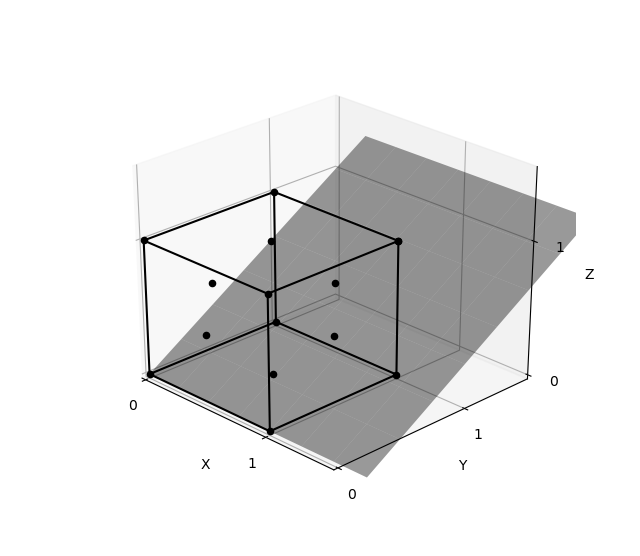
\includegraphics[width=0.6\linewidth]{Graphics/Chapter1/PLANE032}
	\caption{$(0\overline{3}2)$-Plane in a FCC-Lattice}
	\label{}
\end{figure}


\begin{figure}[H]
	\centering
	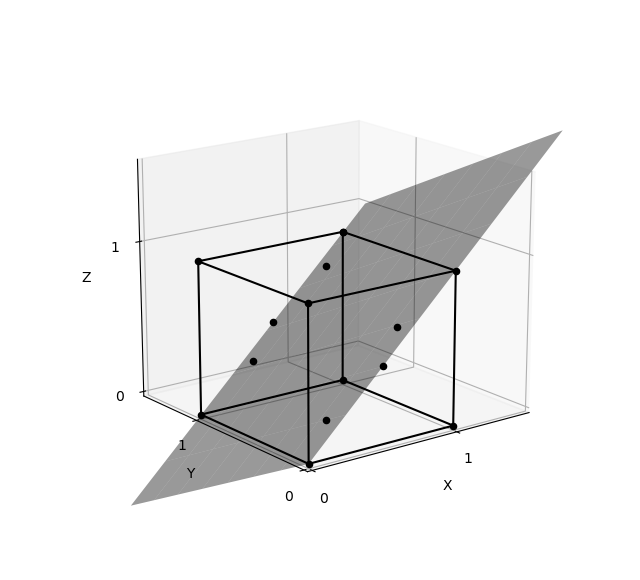
\includegraphics[width=0.6\linewidth]{Graphics/Chapter1/PLANE121}
	\caption{$(\overline{1}21)$-Plane in a FCC-Lattice}
	\label{}
\end{figure}


\subsubsection*{Linear Density [110]}

\begin{figure}[H]
	\centering
	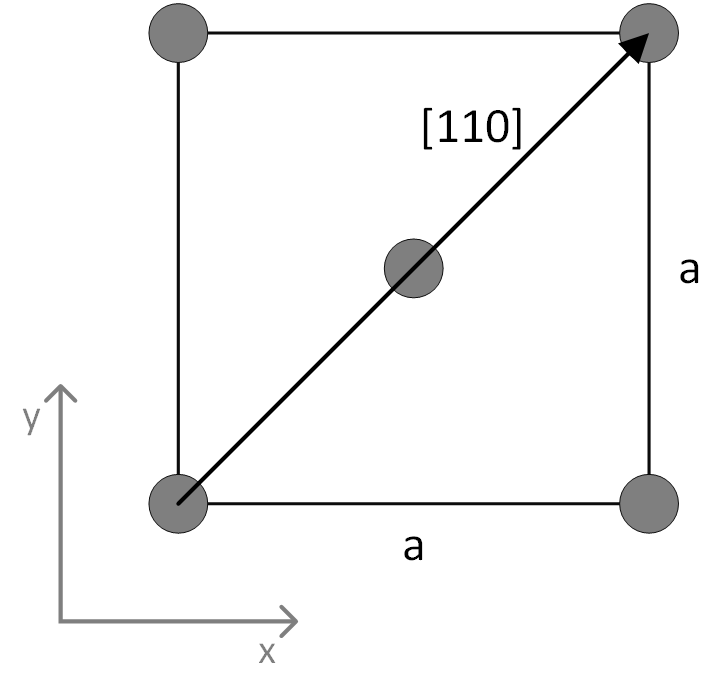
\includegraphics[width=0.5\linewidth]{Graphics/Chapter1/Lin_Den}
	\caption{Linear Density of FCC in [110] Direction}
	\label{fig:Lin_Den}
\end{figure}

\autoref{fig:Lin_Den} shows the [110] direction in a FCC lattice.
As you can see the [110] direction includes 2 atoms inside a 
length of $\sqrt{2}a$.

Therefore  (with $a = 5.56 \, \mathring{A}$)

$$\lambda = \frac{2 \, Atoms}{\sqrt{2}a} = \frac{\sqrt{2}}{5.56} \frac{Atoms}{\mathring{A}}$$

\subsubsection*{Potential Energy}

The potential energy between to adjacent ions can be represented by:

\begin{equation}
	E(r) = - \frac{A}{r} + \frac{B}{r^n}
	\label{eq:Pot_Energy}
\end{equation}


To calculate the bonding energy $E_0 = E(r_0)$, which is a minimum of the function $E(r)$,
the derivative has to equals zero.
The negative derivative of the bonding energy equals the interatomic force.

$$F(r) = - \frac{\partial E(r)}{\partial r} = 0$$

$$-\frac{A}{r^2} + \frac{nB}{r^{n+1}} = 0$$
$$\Rightarrow r_0 = \left( \frac{A}{nB} \right)^{\frac{1}{n-1}}$$

By inserting the result for $r_0$ into \autoref{eq:Pot_Energy}, the bonding energy $E_0$ in terms of $A$, $B$ and $n$ results as:

$$E_0 = E(r_0) = - \frac{A}{\left( \frac{A}{nB} \right)^{\frac{1}{n-1}}} + 
				\frac{B}{\left( \frac{A}{nB} \right)^{\frac{n}{n-1}}}$$

